% Preamble
\documentclass[a4paper, 12pt]{article}
\usepackage[margin=1in]{geometry} % Set margin
\usepackage{pdfpages} % Insert pdf pages
\usepackage{amssymb,amsmath,amsthm, amsfonts} % Math libraries

% Line spacing
\usepackage{setspace}
\setstretch{1.4}

% Custom commands
\newcommand{\sub}[1]{\subsection{\underline{#1}}}
\newcommand{\subsub}[1]{\subsubsection{\underline{#1}}}
\newcommand{\?}{\stackrel{?}{=}}
\newcommand{\R}{\ensuremath{\mathbb{R}}}
\newcommand{\F}{\ensuremath{\mathbb{F}}}
\newcommand{\eqbcuz}[1]{\text{~$\stackrel{(#1)}{=}$~}}
\renewcommand{\qed}{\ensuremath{\hfill\blacksquare\pagebreak}}
\renewcommand{\b}[1]{\textbf{#1}}
\renewcommand{\because}[1]{~\b{(#1)}\\}
\renewcommand{\d}{\ensuremath{\Downarrow\\~}}

% Begin Document %
\begin{document}

% Title Page
\begin{titlepage}
    %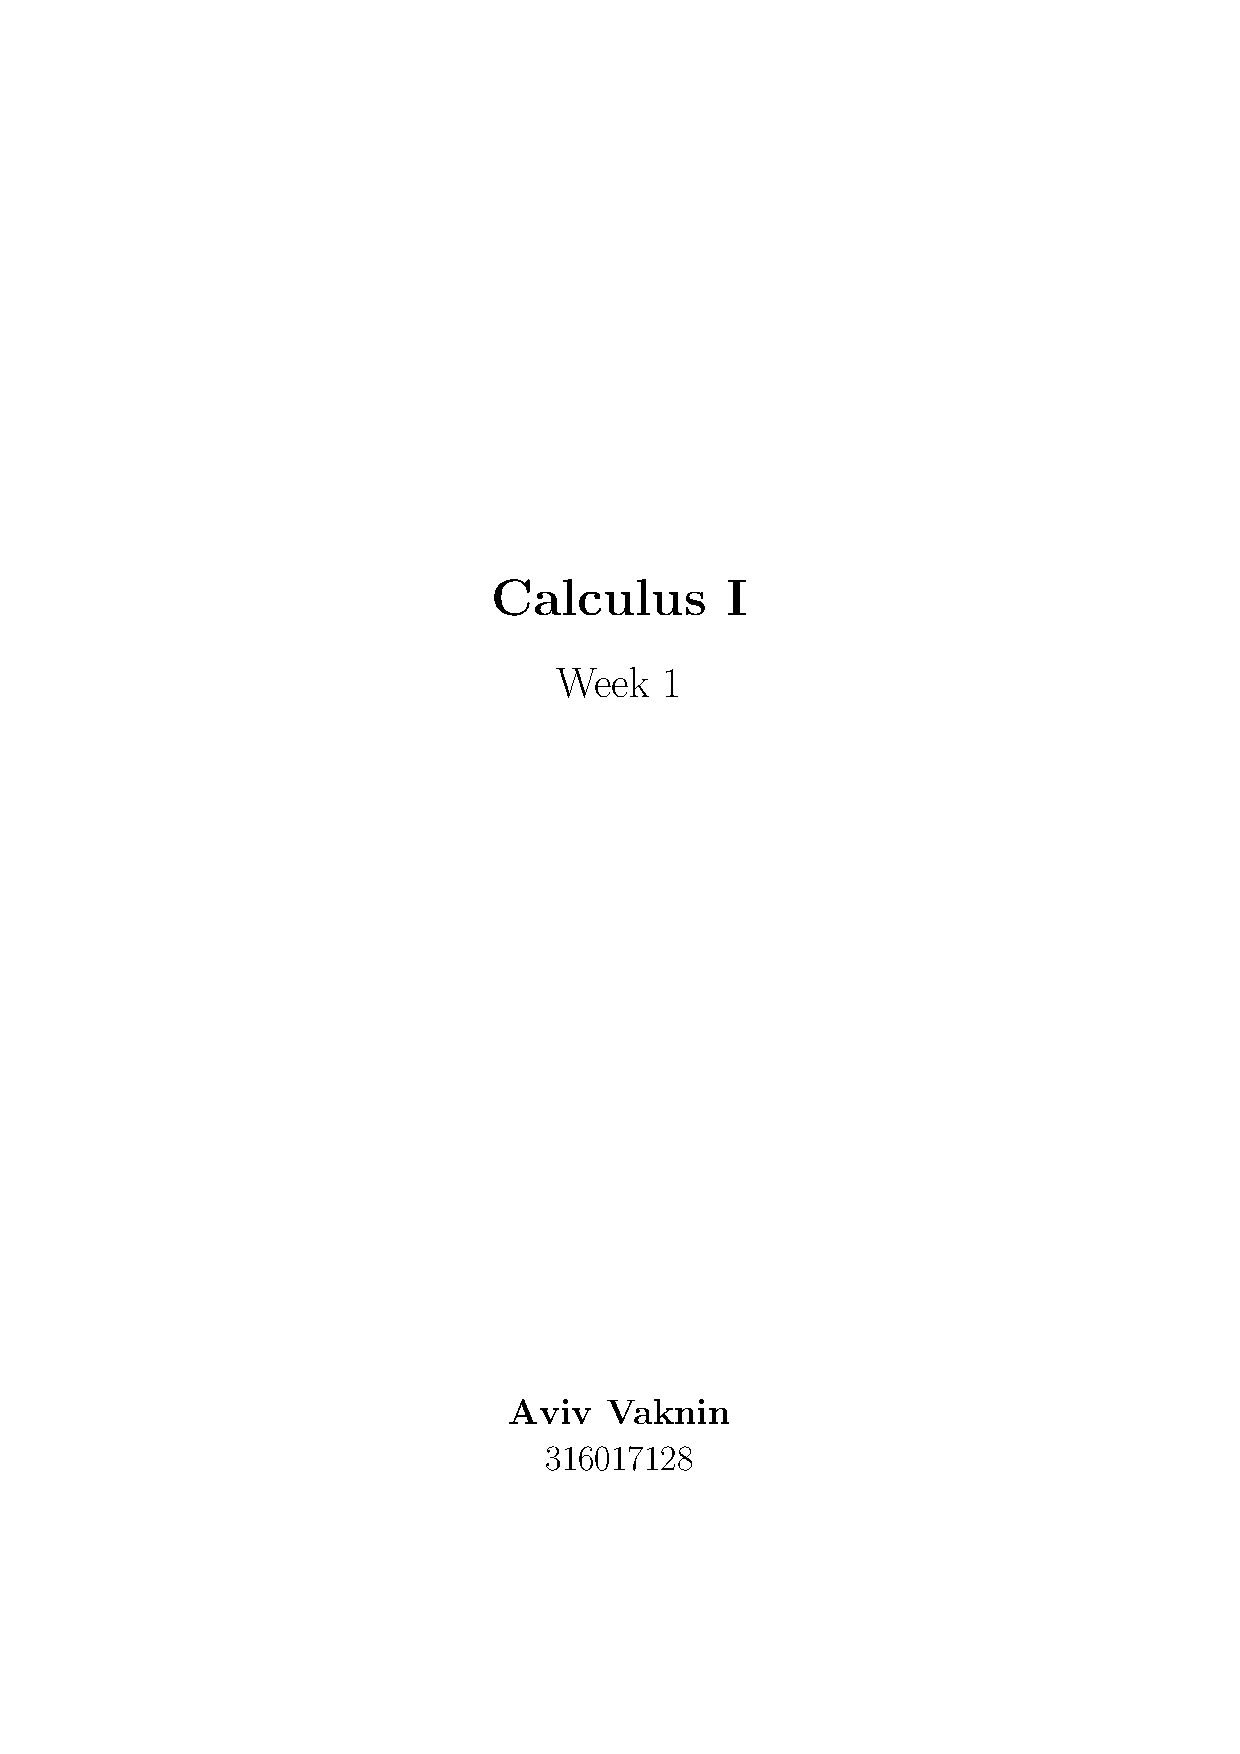
\includepdf{title.pdf}
\end{titlepage}

\section{}
\sub{}
While $i$ and $ii$ are statements, $iii$ isn't a statement,\\
because we haven't received any information about $x$'s value.
\sub{}
    \textit{i})\\
        Statement: $$ \forall{n}\in{\F} ~~ \exists{m}\in{\F} ~\big{|}~ n=m+m $$
        Negated Statement: $$ \exists{n}\in{\F} ~~ \forall{m}\in{\F} ~\big{|}~ n\neq m+m $$
    \textit{ii})\\
        Statement: $$ \forall{m,n}\in{\F} ~~ n=m+m \rightarrow -n=-m-m $$
        Negated Statement: $$ \exists{m,n}\in{\F} ~~ n=m+m ~\land~ -n\neq-m-m $$
\sub{}
    \textit{i})\\
        Statement: $$ \forall{n}\in{\F} ~~ \exists{m}\in{\F} ~\big{|}~ n=m+m $$
        Negated Statement: $$ \exists{n}\in{\F} ~~ \forall{m}\in{\F} ~\big{|}~ n\neq m+m $$


% End
\end{document}